%%%%%%%%%%%%%%%%%%%%%%%%%%%%%%%%%%%%%%%%%%%%%%%%%%%%%%%%%%%%%%%%%%%%%%
% Problem statement
\begin{statement}[
  problempoints=100,
  timelimit=1 sekunda,
  memorylimit=512 MiB,
]{Pastiri}

,,\textit{Nikada nisam bio toliko sit da nisam mogao pojesti još kilu janjetine.}''
  -- gosp. M.

Stado od $K$ ovaca živi na stablu, tj. jednostavnom povezanom grafu bez ciklusa
koji se sastoji od $N$ vrhova.
U svakom vrhu stabla živi najviše jedna ovca.
Stara narodna mudrost kaže: ,,\textit{vukovi
se kriju i \sout{piju} jedu ti ovce.}'' 

Kako bismo obranili naše ovce od zlih
vukova, potrebno je u neke vrhove stabla postaviti pastire, tako da svaku
ovcu čuva barem jedan pastir. Poznato je da \textbf{svaki pastir čuva sve
sebi najbliže ovce}, i samo njih. Također, pastir se može nalaziti u istom vrhu
kao i neka ovca, dakako, tada on čuva samo tu ovcu.

Odredite \textbf{najmanji broj pastira} koje je potrebno postaviti u vrhove danog
stabla tako da \textbf{svaku ovcu čuva barem jedan pastir}. Dodatno, odredite neki takav
raspored najmanjeg mogućeg broja pastira.

%%%%%%%%%%%%%%%%%%%%%%%%%%%%%%%%%%%%%%%%%%%%%%%%%%%%%%%%%%%%%%%%%%%%%%
% Input
\subsection*{Ulazni podaci}
U prvom su retku prirodni brojevi $N$ i $K$ $(1 \le K \le N)$ iz teksta zadatka.

U sljedećih $N-1$ redaka nalaze se po dva prirodna broja $a_i$ i $b_i$ $(1 \le a_i, b_i \le N)$ koji
označavaju da postoji neusmjerena veza u stablu između vrhova s oznakama $a_i$ i $b_i$.

U sljedećem se retku nalazi $K$ različitih prirodnih brojeva $o_i$ $(1 \le o_i \le N)$ koji
predstavljaju oznake čvorova u kojima se nalaze ovce.

%%%%%%%%%%%%%%%%%%%%%%%%%%%%%%%%%%%%%%%%%%%%%%%%%%%%%%%%%%%%%%%%%%%%%%
% Output
\subsection*{Izlazni podaci}
U prvom retku ispišite broj $X$, koji predstavlja najmanji mogući broj pastira
iz teksta zadatka.

U drugom retku ispišite $X$ brojeva odvojenih razmakom, koji predstavljaju oznake
čvorova u koje treba postaviti pastire.

%%%%%%%%%%%%%%%%%%%%%%%%%%%%%%%%%%%%%%%%%%%%%%%%%%%%%%%%%%%%%%%%%%%%%%
% Scoring
\subsection*{Bodovanje}
{\renewcommand{\arraystretch}{1.4}
  \setlength{\tabcolsep}{6pt}
  \begin{tabular}{ccl}
 Podzadatak & Broj bodova & Ograničenja \\ \midrule
  1 & 8 & $1 \le N \le 500\,000$, svaki vrh $x = 1, \dots, n-1$ je povezan s vrhom $x + 1$\\
  2 & 18 & $1 \le K \le $ \textbf{TODO}, $\, 1 \le N \le 500\,000$ \\
  3 & 23 & $1 \le N \le $ \textbf{TODO} \\
  4 & 51 & $1 \le N \le 500\,000$ \\
\end{tabular}}

%%%%%%%%%%%%%%%%%%%%%%%%%%%%%%%%%%%%%%%%%%%%%%%%%%%%%%%%%%%%%%%%%%%%%%
% Examples
\subsection*{Probni primjeri}
\begin{tabularx}{\textwidth}{X'X'X}
\sampleinputs{test/pastiri.dummy.in.1}{test/pastiri.dummy.out.1} &
\sampleinputs{test/pastiri.dummy.in.2}{test/pastiri.dummy.out.2} &
\sampleinputs{test/pastiri.dummy.in.3}{test/pastiri.dummy.out.3}
\end{tabularx}

\textbf{Pojašnjenje trećeg probnog primjera:}
\begin{figure}[H]
\centering
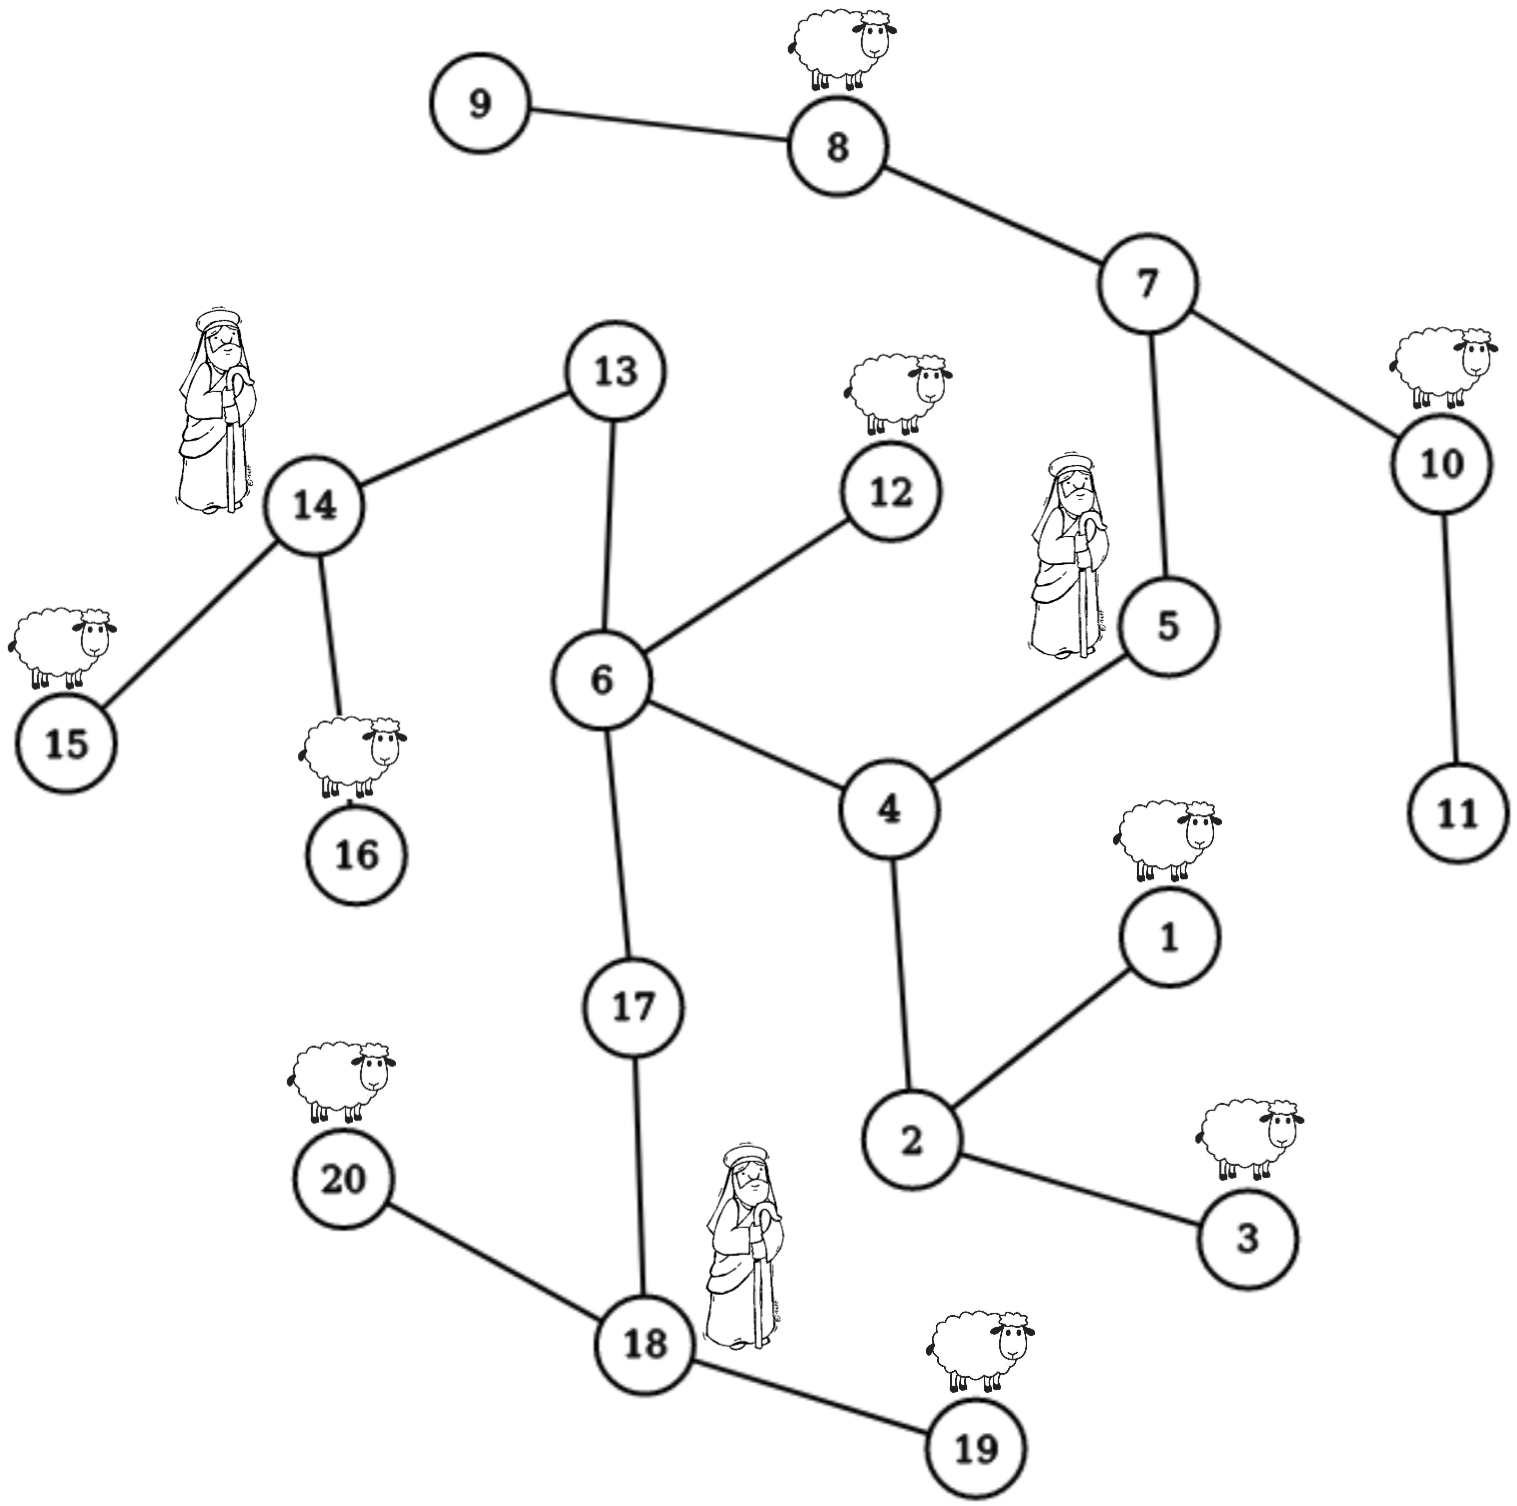
\includegraphics[width=0.57\textwidth]{img/pastiri_tp.png}
\end{figure}

%%%%%%%%%%%%%%%%%%%%%%%%%%%%%%%%%%%%%%%%%%%%%%%%%%%%%%%%%%%%%%%%%%%%%%
% We're done
\end{statement}

%%% Local Variables:
%%% mode: latex
%%% mode: flyspell
%%% ispell-local-dictionary: "croatian"
%%% TeX-master: "../hio.tex"
%%% End:
